\section{Trajectory Planning}

At this step, given the points of the desired path, a more detailed trajectory is calculated, 
which will contain all the waypoints that the robot will have to visit. Trajectory planning is executed after a desired path is generated,
and consists in mapping the geometric points to specific \textbf{time points}, as well as assigning specific \textbf{velocities}, \textbf{accelerations} and \textbf{jerks}, 
in order to generate the commands needed for the robot controller to execute a smooth motion.

In chapter \ref{subsection:pivot-motions}, the paths that are calculated are parameterized by the path parameter $s$. As $s$ increases from $0$, the robot moves from the start configuration $q(0)$ to the goal configuration $q(1)$. 
Path planning outputs geometric information $q(s), s \in [0, 1]$, whereas the \textbf{trajectories} that are the subject of this chapter, also include \textbf{time information} $q(t), t \in [0, T]$. 
A path can be converted to a trajectory by defining a function $s(t): [0, T] \rightarrow [0, 1]$ which maps the time parameter's range to the path parameter's range. This function is also known as \textbf{time scaling} or 
\textbf{time parameterization}.

The most common methodology of trajectory planning, which is also used in this thesis, is the one that is studied in the \textbf{joint angles space} also known as \textbf{configuration space}.

\subsection{Trajectory planning in joint angles space}

\begin{center}
\begin{figure}[H]
\centering
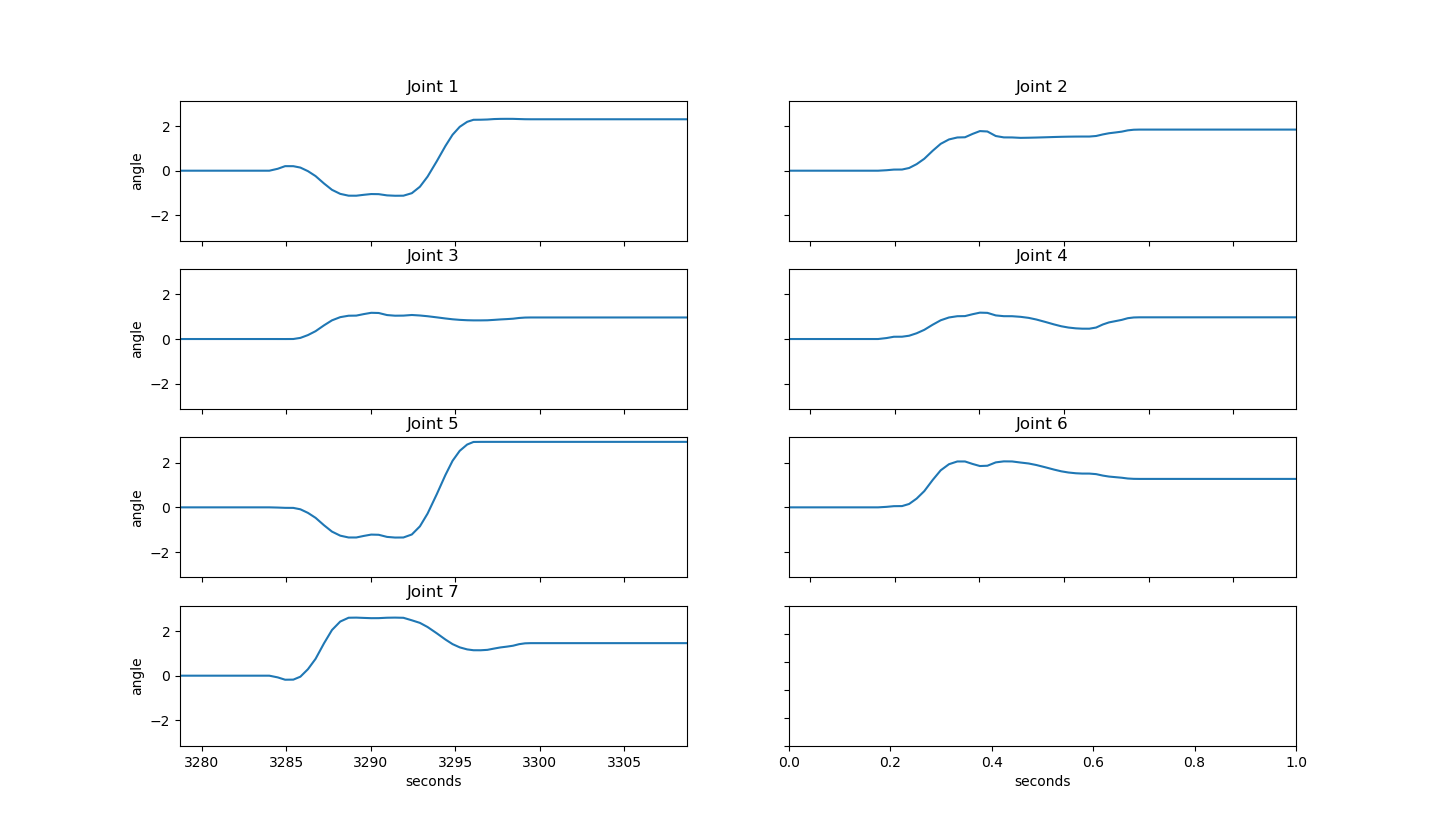
\includegraphics[width=\textwidth]{images/trajectory1-test1.png}\\
\caption{Trajectory diagrams in joints space.}
\end{figure}
\end{center}


\subsubsection{Polynomials of 5th order}


\subsubsection{Trapezoidal velocity profile}


\subsubsection{S-Curve velocity profile}


\subsection{Trajectory planning in cartesian coordinates}

Connect the points from path planning with line segments and add more points if needed

\begin{center}
\begin{figure}[H]
\centering
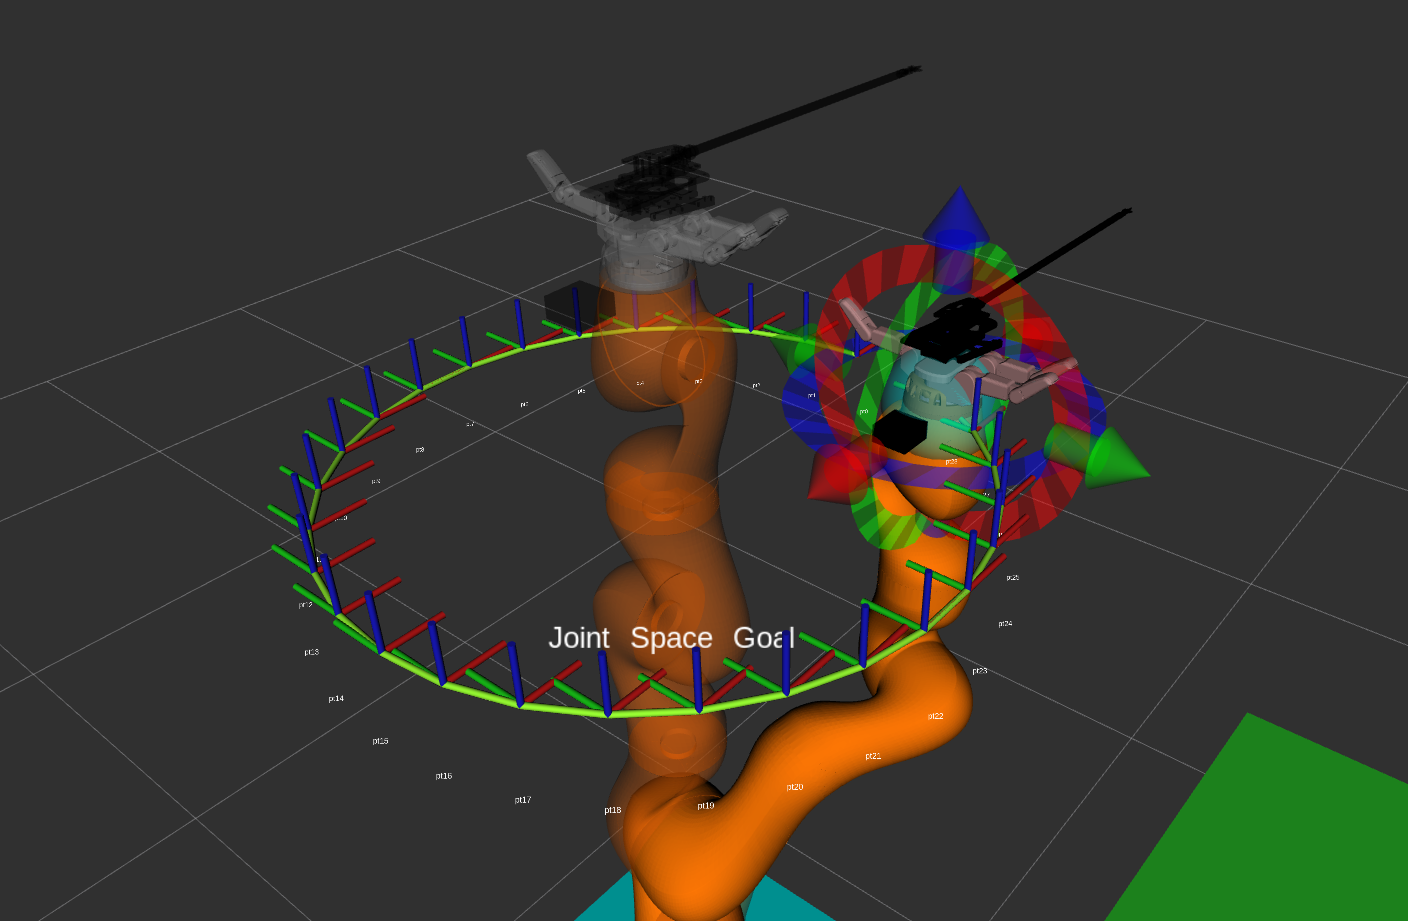
\includegraphics[width=0.7\textwidth]{images/simple_circular_traj1.png}\\
\caption{Circlular trajectory around the z axis of the home position of the robot}
\label{fig:circ-traj-out-of-angle-range}
\end{figure}
\end{center}

It is very important that the designed trajectory respects the joints angles' range. For example
depending on the starting position of the circular trajectory depicted at figure 
\ref{fig:circ-traj-out-of-angle-range}, the robot arm may reach it's joint bounds and in order to 
continue executing the trajectory it will have to make a sudden jump to reset the angles. 
This could have serious side-effects for both the surgical task and thus the patient, as well as 
for the operating staff, who control the robot.